% Options for packages loaded elsewhere
\PassOptionsToPackage{unicode}{hyperref}
\PassOptionsToPackage{hyphens}{url}
%
\documentclass[
  12pt,
  man, donotrepeattitle]{apa6}
\usepackage{amsmath,amssymb}
\usepackage{lmodern}
\usepackage{iftex}
\ifPDFTeX
  \usepackage[T1]{fontenc}
  \usepackage[utf8]{inputenc}
  \usepackage{textcomp} % provide euro and other symbols
\else % if luatex or xetex
  \usepackage{unicode-math}
  \defaultfontfeatures{Scale=MatchLowercase}
  \defaultfontfeatures[\rmfamily]{Ligatures=TeX,Scale=1}
  \setmainfont[]{Times New Roman}
\fi
% Use upquote if available, for straight quotes in verbatim environments
\IfFileExists{upquote.sty}{\usepackage{upquote}}{}
\IfFileExists{microtype.sty}{% use microtype if available
  \usepackage[]{microtype}
  \UseMicrotypeSet[protrusion]{basicmath} % disable protrusion for tt fonts
}{}
\makeatletter
\@ifundefined{KOMAClassName}{% if non-KOMA class
  \IfFileExists{parskip.sty}{%
    \usepackage{parskip}
  }{% else
    \setlength{\parindent}{0pt}
    \setlength{\parskip}{6pt plus 2pt minus 1pt}}
}{% if KOMA class
  \KOMAoptions{parskip=half}}
\makeatother
\usepackage{xcolor}
\usepackage{graphicx}
\makeatletter
\def\maxwidth{\ifdim\Gin@nat@width>\linewidth\linewidth\else\Gin@nat@width\fi}
\def\maxheight{\ifdim\Gin@nat@height>\textheight\textheight\else\Gin@nat@height\fi}
\makeatother
% Scale images if necessary, so that they will not overflow the page
% margins by default, and it is still possible to overwrite the defaults
% using explicit options in \includegraphics[width, height, ...]{}
\setkeys{Gin}{width=\maxwidth,height=\maxheight,keepaspectratio}
% Set default figure placement to htbp
\makeatletter
\def\fps@figure{htbp}
\makeatother
\setlength{\emergencystretch}{3em} % prevent overfull lines
\providecommand{\tightlist}{%
  \setlength{\itemsep}{0pt}\setlength{\parskip}{0pt}}
\setcounter{secnumdepth}{-\maxdimen} % remove section numbering
% Make \paragraph and \subparagraph free-standing
\ifx\paragraph\undefined\else
  \let\oldparagraph\paragraph
  \renewcommand{\paragraph}[1]{\oldparagraph{#1}\mbox{}}
\fi
\ifx\subparagraph\undefined\else
  \let\oldsubparagraph\subparagraph
  \renewcommand{\subparagraph}[1]{\oldsubparagraph{#1}\mbox{}}
\fi
\newlength{\cslhangindent}
\setlength{\cslhangindent}{1.5em}
\newlength{\csllabelwidth}
\setlength{\csllabelwidth}{3em}
\newlength{\cslentryspacingunit} % times entry-spacing
\setlength{\cslentryspacingunit}{\parskip}
\newenvironment{CSLReferences}[2] % #1 hanging-ident, #2 entry spacing
 {% don't indent paragraphs
  \setlength{\parindent}{0pt}
  % turn on hanging indent if param 1 is 1
  \ifodd #1
  \let\oldpar\par
  \def\par{\hangindent=\cslhangindent\oldpar}
  \fi
  % set entry spacing
  \setlength{\parskip}{#2\cslentryspacingunit}
 }%
 {}
\usepackage{calc}
\newcommand{\CSLBlock}[1]{#1\hfill\break}
\newcommand{\CSLLeftMargin}[1]{\parbox[t]{\csllabelwidth}{#1}}
\newcommand{\CSLRightInline}[1]{\parbox[t]{\linewidth - \csllabelwidth}{#1}\break}
\newcommand{\CSLIndent}[1]{\hspace{\cslhangindent}#1}
\ifLuaTeX
\usepackage[bidi=basic]{babel}
\else
\usepackage[bidi=default]{babel}
\fi
\babelprovide[main,import]{english}
% get rid of language-specific shorthands (see #6817):
\let\LanguageShortHands\languageshorthands
\def\languageshorthands#1{}
% Manuscript styling
\usepackage{upgreek}
\captionsetup{font=singlespacing,justification=justified}

% Table formatting
\usepackage{longtable}
\usepackage{lscape}
% \usepackage[counterclockwise]{rotating}   % Landscape page setup for large tables
\usepackage{multirow}		% Table styling
\usepackage{tabularx}		% Control Column width
\usepackage[flushleft]{threeparttable}	% Allows for three part tables with a specified notes section
\usepackage{threeparttablex}            % Lets threeparttable work with longtable

% Create new environments so endfloat can handle them
% \newenvironment{ltable}
%   {\begin{landscape}\centering\begin{threeparttable}}
%   {\end{threeparttable}\end{landscape}}
\newenvironment{lltable}{\begin{landscape}\centering\begin{ThreePartTable}}{\end{ThreePartTable}\end{landscape}}

% Enables adjusting longtable caption width to table width
% Solution found at http://golatex.de/longtable-mit-caption-so-breit-wie-die-tabelle-t15767.html
\makeatletter
\newcommand\LastLTentrywidth{1em}
\newlength\longtablewidth
\setlength{\longtablewidth}{1in}
\newcommand{\getlongtablewidth}{\begingroup \ifcsname LT@\roman{LT@tables}\endcsname \global\longtablewidth=0pt \renewcommand{\LT@entry}[2]{\global\advance\longtablewidth by ##2\relax\gdef\LastLTentrywidth{##2}}\@nameuse{LT@\roman{LT@tables}} \fi \endgroup}

% \setlength{\parindent}{0.5in}
% \setlength{\parskip}{0pt plus 0pt minus 0pt}

% Overwrite redefinition of paragraph and subparagraph by the default LaTeX template
% See https://github.com/crsh/papaja/issues/292
\makeatletter
\renewcommand{\paragraph}{\@startsection{paragraph}{4}{\parindent}%
  {0\baselineskip \@plus 0.2ex \@minus 0.2ex}%
  {-1em}%
  {\normalfont\normalsize\bfseries\itshape\typesectitle}}

\renewcommand{\subparagraph}[1]{\@startsection{subparagraph}{5}{1em}%
  {0\baselineskip \@plus 0.2ex \@minus 0.2ex}%
  {-\z@\relax}%
  {\normalfont\normalsize\itshape\hspace{\parindent}{#1}\textit{\addperi}}{\relax}}
\makeatother

% \usepackage{etoolbox}
\makeatletter
\patchcmd{\HyOrg@maketitle}
  {\section{\normalfont\normalsize\abstractname}}
  {\section*{\normalfont\normalsize\abstractname}}
  {}{\typeout{Failed to patch abstract.}}
\patchcmd{\HyOrg@maketitle}
  {\section{\protect\normalfont{\@title}}}
  {\section*{\protect\normalfont{\@title}}}
  {}{\typeout{Failed to patch title.}}
\makeatother

\usepackage{xpatch}
\makeatletter
\xapptocmd\appendix
  {\xapptocmd\section
    {\addcontentsline{toc}{section}{\appendixname\ifoneappendix\else~\theappendix\fi\\: #1}}
    {}{\InnerPatchFailed}%
  }
{}{\PatchFailed}
\keywords{Up,to,eight,keywords\newline\indent Word count: X}
\DeclareDelayedFloatFlavor{ThreePartTable}{table}
\DeclareDelayedFloatFlavor{lltable}{table}
\DeclareDelayedFloatFlavor*{longtable}{table}
\makeatletter
\renewcommand{\efloat@iwrite}[1]{\immediate\expandafter\protected@write\csname efloat@post#1\endcsname{}}
\makeatother
\usepackage{lineno}

\linenumbers
\usepackage{csquotes}
\usepackage{float}
\floatplacement{figure}{H}
\usepackage{booktabs}
\usepackage{setspace}
\raggedbottom
\usepackage{tabu}
\usepackage{makecell}
\usepackage{pdflscape}
\usepackage{longtable}
\newcommand{\blandscape}{\begin{landscape}}
\newcommand{\elandscape}{\end{landscape}}
\setlength\parindent{22pt}
\ifLuaTeX
  \usepackage{selnolig}  % disable illegal ligatures
\fi
\IfFileExists{bookmark.sty}{\usepackage{bookmark}}{\usepackage{hyperref}}
\IfFileExists{xurl.sty}{\usepackage{xurl}}{} % add URL line breaks if available
\urlstyle{same} % disable monospaced font for URLs
\hypersetup{
  pdftitle={Is there really such a thing as Tropical Biology?},
  pdfauthor={Emilio M. Bruna1,2,3},
  pdflang={en-EN},
  pdfkeywords={Up,to,eight,keywords},
  hidelinks,
  pdfcreator={LaTeX via pandoc}}

\title{Is there really such a thing as \emph{Tropical} Biology?}
\author{Emilio M. Bruna\textsuperscript{1,2,3}}
\date{}


\shorttitle{Draft for \emph{Biotropica}}

\authornote{

Received:\_\_\_\_\_\_; Revised:\_\_\_\_\_\_; Accepted:\_\_\_\_\_\_.

}

\affiliation{\vspace{0.5cm}\textsuperscript{1} Department of Wildlife Ecology and Conservation, University of Florida, PO Box 110430, Gainesville, FL 32611-0430, USA\\\textsuperscript{2} Center for Latin American Studies, University of Florida, PO Box 115530, Gainesville, FL 32611-5530, USA}

\begin{document}
\maketitle

\onehalfspacing
\singlespacing

\begin{quote}
``There are few things more presumptuous than a US scientist holding forth on the future of tropical ecology'' (Janzen 1972).
\end{quote}

\hypertarget{introduction}{%
\subsection{1. INTRODUCTION}\label{introduction}}

\begin{enumerate}
\def\labelenumi{\arabic{enumi}.}
\tightlist
\item
  Motivation: In 19XX I received a decision on a manuscript that included justification I suspect many of us have seen:
\end{enumerate}

\begin{quote}
\begin{quote}
''The scope of your paper makes it more appropriate for a specialized journal focusing on tropical systems''
\end{quote}
\end{quote}

\begin{enumerate}
\def\labelenumi{\arabic{enumi}.}
\item
  This has always trouybled me, because there is an implicit (or explicit) emphasis in training students and professional advancement that broad, general conclusions should be our scientific goal. The implication of this decision is that those of us that call ourselves tropical biologists are making a less general (=less important) contribution.
\item
  In recent years we have seen the re-emergence of what is actually an old conversation - the extent to which not tropical biologists, but biologists from tropical countries are excluded from the scientific process.
\item
  Here I reconsider the notion that Tropical Biology is a specialized discipline of the biological sciences by considering two distinct but related datasets - the way in which biologists self-organize into specialized groups (i.e., subdisciplines) and (2) the topics of their research and how the way in which they conceptualize their contributions to the scientific literature.
\item
  I wish to emphasize that this is by no means intended to be a comprehensive historical overview of the field. Nor am I the first to have wrestled with questions about the breadth, novelty, and status of tropical biology (Robinson 1978, Zuk 2016, Janzen n.d.).
\end{enumerate}

Instead, my goal is to stimulate discussion about the fundamental yet generally ignored question that serves as the foundation on which our association is built: Is there really such a thing as \emph{``Tropical''} Biology?

\hypertarget{why-the-answer-might-be-no}{%
\subsection{\texorpdfstring{1. Why the answer might be \emph{`No'}}{1. Why the answer might be `No'}}\label{why-the-answer-might-be-no}}

\begin{enumerate}
\def\labelenumi{\arabic{enumi}.}
\item
  There are different way in which\\
\item
  This specialization could be one of (specialization of approach and tools, conceptual domain, or study system). Figure 1.
\item
  `Tropical' transcends all of these.
\item
  Moreover, the tropics is transcendent: tropical species don't stop at the 23rd parallel, the adjective is rarely used in the tropics themselves, and although ``tropics'' has a very specific definition, biologists rarely use it\ldots in fact, they don;t have a consistent definition.
\item
  The fact is that ``the tropics'' as a distinct and unique entity is a historical artefact whose end result was considering the tropics as (culturally, scientifically, biologically) `other' and `unique'.
\end{enumerate}

Tropical biology defies all of these specialization guidelines.
It is cross-conceptual, cross-tool, and cross-system - it simply doesn't fit neatly into any of these specialization categories along which scholars typically self-organize.

But perhaps the best evidence that there really isn't such a thing as Tropical Biology is that the term is primarily used \emph{outdside} of the tropics. It is rare for colleges in Brazil or India or Peru to offer a course in ``Tropical Biology'' or ``Tropical Ecology'' - they simply call it ``Ecology''.

The tropics also defy biological definition - the distributions of ``tropical'' species don't end at the 23rd parallels.

Finally, even tropical biologists can't agree on what the tropics are - Feeley and Stroud surveyed the literature and found that biologists working in the tropics defined the region at least eight different ways (Feeley \& Stroud 2018).

The reason for this divergence is that the tropics exist as an astronomical artefact - they are the points on earth that are exposed to directly overhead solar radiation for at least one day.

Their existence in the colloquial sense - as a distinct region - is actually a historical artifact that traces its origins back to Marco Polo. He was not the first european to visit the tropics in search of spices like cinnamon and nutmeg, but he was the first person whose vivid descriptions about the things he saw mesmerized European audiences. Over the course of the next several centuries, these stories were retold, reinterpreted, and mixed with the stories of others to cement in our imaginations multiple paradigms defining the tropics and the people that lived there.

\hypertarget{why-the-answer-might-be-maybe}{%
\subsection{\texorpdfstring{2. Why the answer might be \emph{`Maybe'}}{2. Why the answer might be `Maybe'}}\label{why-the-answer-might-be-maybe}}

\begin{enumerate}
\def\labelenumi{\arabic{enumi}.}
\item
  Despite its origins as a colonial construct, Tropical Biology could still be a conceptually distinct field if the scientists studying tropical systems address a distinct suite of topics than those working in other regions.
\item
  To assess this possibility, I compared the titles and keywords of articles published from 1960-2022 four `Tropical Journals' (\emph{Journal of Tropical Ecology}, \emph{Biotropica}, \emph{Tropical Ecology}, and \emph{Tropical Conservation Science}) with those of research from both tropical and extra-tropical locations that had been published in six `General Journals' (\emph{The American Naturalist}, \emph{Evolution}, \emph{Journal of Evolutionary Biology}, \emph{Journal of Ecology}, \emph{Ecology}, and \emph{Journal of Animal Ecology})
\item
  (N=62,750 and N = 220,612, respectively)
\end{enumerate}

I found that 10 of the top 20 key words for articles published in ``Tropical Journals'' were either a geographic location (e.g., \emph{Costa Rica}, \emph{Amazonia}) or the ecosystem in which the study was conducted (e.g., \emph{tropical dry forest}, \emph{savanna}).

In contrast, the the 20 most common key words in the ``General Journals'' were conceptual (e.g., \emph{compeititon}, \emph{species diversity}, \emph{climate change}, \emph{sexual selection}). The exception were articles based on research conducted in the tropics, which also emphasized the location or system.

The only overlap is in\ldots.

Article titles show a similar pattern - the most bi-grams for ``Tropical Journals'' were almost all about the study system, whereas in Global Journals they were conceptual with three notable exceptions: \emph{Drosophila melanogaster}, \emph{plant/tree species/communities}, and \emph{rain forest}.

\emph{Drosophila melangoaster} is one of the most important model systems for experimental work investigating evolutionary processes, and plant communities have been a major focus of research since the pioneering work of Clemments and Gleason. Of this work, only tropical forests get a descriptive adjective.

(Anon n.d.a)

While preliminary, this suggests

Discussion \& Caveats

\hypertarget{why-the-answer-might-be-yes}{%
\subsection{\texorpdfstring{3. Why the answer might be \emph{`Yes'}}{3. Why the answer might be `Yes'}}\label{why-the-answer-might-be-yes}}

What makes 'Tropical Biology'' distinct is not the science \emph{per se}, but rather then broader context in which that science is conducted. Research anywhere can be difficult, but for most tropical biologists the daily struggle with precarious infrastructure, economic volatility, drastically reduced funding for research and education, and political instability can feel insurmountable - and all this is before having to communicate one's results in a foreign language to the potentially biased reviewers (Anon n.d.b) and readers of journals that charge open access fees equivalent to several months salary. When added to the physical and emotional toll of disease, crime, working in isolation, field sites being cleared at unprecedented rates, and threats of professional retribution or physical violence, tropical biology and conservation can be uniquely dangerous - even deadly. Lamentably, this is also true for the truly heroic environmental journalists and advocates with whom we collaborate.

\hypertarget{the-future-of-tropical-biology}{%
\subsection{4. The Future of (Tropical) Biology}\label{the-future-of-tropical-biology}}

How then to resolve this conundrum? I believe that the solution is neither dropping the adjective that inspires so many of us, nor keeping it and accepting status as complementary subdiscipline. Instead, I call on our members to \textbf{\emph{reclaim and reshape the Tropical narrative}} by continuing to emphasize what makes tropical biology distinct - place and context - while also repositioning tropical ecosystems as the biological baseline. Here are six simple ways that anyone can contribute to this movement:

\begin{enumerate}
\def\labelenumi{\arabic{enumi}.}
\item
  \textbf{\emph{Cite with purpose.}} Citation is a powerful and political act: it conveys legitimacy on the scholarship in the article being cited as well as its author, helps elevate the profile of the author and study system, and those reading your work will cite these articles when writing their own. For many scientists it also plays an important role in their professional advancement. Be mindful of this power and the opportunity it presents when choosing which articles to cite. Cite scientists whose work or approach you feel is undervalued or overlooked. Cite scientists from countries or institutions that have been ignored by the broader scientific community. Cite scientists whose approach to research you feel others should emulate. Cite studies conducted in the tropics.
\item
  \textbf{\emph{Teach with Purpose.}} All tropical biologists are teachers, whether it be in a classroom or in a meeting with policy makers, and teaching also provides an opportunity to elevate the scholarship of others. Be mindful of whose papers are assigned as readings, the studies and systems used to illustrate concepts, the scientists highlighted in presentations, and who is invited to speak in seminar series or present guest lectures. Use your syllabus as a tool to recast the biological narrative about tropical ecosystems and the composition of the scientific community that studies them. Train students in the skills needed when working in tropical systems - collaboration, facilitation, conflict resolution, and communication to diverse audiences (Kainer \emph{et al.} 2006, Duchelle \emph{et al.} 2009).
\item
  \textbf{\emph{Collaborate with Purpose.}} Helicopter science. International collaboration can be challenging, but the results are often published in more prestigious outlets and have higher citation rates (Smith \emph{et al.} 2014). treating coauthorship is collaboration. Purposeful collaboration requires Allow community members to guide the identification of research questions (Kainer \emph{et al.} 2009). Push for organizations to strengthen collaborations within the Global South.
\item
  \textbf{\emph{Build on public fascination with the tropics.}} Public fascination with the tropics and their charismatic species (Albert \emph{et al.} 2018) provides unparalleled opportunities for outreach and education (Moreira \& Robles 2017). Global events like the World Cup (Melo \emph{et al.} 2014), teams with tropical species as mascots (Sartore-Baldwin \& McCullough 2019), movies set in the tropics (Yong \emph{et al.} 2011), tropical images in fashion (Kutesko 2014), viral videos about tropical fruits (Anon n.d.c) - we can find creative ways to leverage this universal appeal into support for tropical research and conservation.
\item
  \textbf{\emph{Get in the Game.}} It's trite, but true - change requires action. Organizations like the ATBC provide myriad opportunities for meaningful engagement. Help make the process of publishing more fair by serving as a review or subject editor for \emph{Biotropica}. Contribute to capacity building efforts by reviewing student seed grants proposals or serving as a judge for student presentations at the annual meeting. Is there an issue about which you are passionate? Join an ATBC committee or chapter and organize a webinar, workshop, hackathon, or reading group on the topic. What should the Association be doing differently? Tell the leadership at the Council Meetings or stand for election and push for change as a Councillor.
\item
  \textbf{\emph{Support and celebrate one another}.} Finally, remember that the work done by tropical biologists addresses the ``neglected problems that afflict most of the world's people'' (Annan 2003) and, regardless of topic, helps advance the socioeconomic condition of the country in which it's conducted. It requires effort and resilience. Seek opportunities to thank and congratulate each other for these contributions - you're truly making the world a better place.
\end{enumerate}

\hypertarget{acknowledgments}{%
\subsection{Acknowledgments}\label{acknowledgments}}

\hypertarget{disclosure-statement}{%
\subsection{Disclosure Statement}\label{disclosure-statement}}

The author confirms that there have been no involvements that might raise the question of bias in the work reported or in the conclusions, implications, or opinions stated.

\newpage

\hypertarget{references}{%
\section{References}\label{references}}

\hypertarget{refs}{}
\begin{CSLReferences}{1}{0}
\leavevmode\vadjust pre{\hypertarget{ref-albertTwentyMostCharismatic2018}{}}%
\textsc{Albert, C.}, \textsc{G. M. Luque}, and \textsc{F. Courchamp}. 2018. The twenty most charismatic species. PLOS ONE 13: e0199149. Available at: \url{https://journals.plos.org/plosone/article?id=10.1371/journal.pone.0199149} {[}Accessed March 14, 2023{]}.

\leavevmode\vadjust pre{\hypertarget{ref-annanChallengeWorldScientists2003}{}}%
\textsc{Annan, K.} 2003. A {Challenge} to the {World}'s {Scientists}. Science 299: 1485--1485. Available at: \url{https://www.science.org/doi/10.1126/science.299.5612.1485} {[}Accessed October 25, 2022{]}.

\leavevmode\vadjust pre{\hypertarget{ref-NorthSouthNaming}{}}%
Anon. North and {South}: {Naming} practices and the hidden dimension of global disparities in knowledge production {\textbar} {PNAS}. Available at: \url{https://www.pnas.org/doi/abs/10.1073/pnas.2119373119} {[}Accessed March 14, 2023a{]}.

\leavevmode\vadjust pre{\hypertarget{ref-PeerReviewPerpetuates}{}}%
Anon. Peer review perpetuates barriers for historically excluded groups {\textbar} {Nature} {Ecology} \& {Evolution}. Available at: \url{https://www.nature.com/articles/s41559-023-01999-w} {[}Accessed March 14, 2023b{]}.

\leavevmode\vadjust pre{\hypertarget{ref-SouthFloridaCouple}{}}%
Anon. South {Florida} couple goes viral on {TikTok}, now selling exotic fruit online -- {WSVN} {7News} {\textbar} {Miami} {News}, {Weather}, {Sports} {\textbar} {Fort} {Lauderdale}. Available at: \url{https://wsvn.com/entertainment/south-florida-couple-goes-viral-on-tiktok-now-selling-exotic-fruit-online/} {[}Accessed March 14, 2023c{]}.

\leavevmode\vadjust pre{\hypertarget{ref-duchelleGraduateStudentsKnowledge2009}{}}%
\textsc{Duchelle, A. E.}, \textsc{K. Biedenweg}, \textsc{C. Lucas}, \textsc{A. Virapongse}, \textsc{J. Radachowsky}, \textsc{D. J. Wojcik}, \textsc{M. Londres}, \textsc{W.-L. Bartels}, \textsc{D. Alvira}, and \textsc{K. A. Kainer}. 2009. Graduate {Students} and {Knowledge} {Exchange} with {Local} {Stakeholders}: {Possibilities} and {Preparation}. Biotropica 41: 578--585. Available at: \url{https://onlinelibrary.wiley.com/doi/abs/10.1111/j.1744-7429.2009.00563.x} {[}Accessed January 26, 2023{]}.

\leavevmode\vadjust pre{\hypertarget{ref-feeleyWhereEarthAre2018}{}}%
\textsc{Feeley, K. J.}, and \textsc{J. T. Stroud}. 2018. Where on {Earth} are the {``tropics''}? Frontiers of Biogeography 10. Available at: \url{https://escholarship.org/uc/item/3vc5s2t3} {[}Accessed June 14, 2022{]}.

\leavevmode\vadjust pre{\hypertarget{ref-janzenWhitherTropicalEcology1972}{}}%
\textsc{Janzen, D.} 1972. Whither {Tropical} {Ecology}. \emph{In} J. A. Behnke (Ed.) Challenging {Biological} {Problems}: {Directions} {Toward} {Their} {Solution}. pp. 281--296, Oxford University Press, New York.

\leavevmode\vadjust pre{\hypertarget{ref-janzenFutureTropicalEcology}{}}%
\textsc{Janzen, D. H.} The future of tropical ecology. 22.

\leavevmode\vadjust pre{\hypertarget{ref-kainerPartneringGreaterSuccess2009}{}}%
\textsc{Kainer, K. A.}, \textsc{M. L. DiGiano}, \textsc{A. E. Duchelle}, \textsc{L. H. O. Wadt}, \textsc{E. Bruna}, and \textsc{J. L. Dain}. 2009. Partnering for {Greater} {Success}: {Local} {Stakeholders} and {Research} in {Tropical} {Biology} and {Conservation}. Biotropica 41: 555--562. Available at: \url{https://onlinelibrary.wiley.com/doi/abs/10.1111/j.1744-7429.2009.00560.x} {[}Accessed January 26, 2023{]}.

\leavevmode\vadjust pre{\hypertarget{ref-kainerGraduateEducationFramework2006}{}}%
\textsc{Kainer, K. A.}, \textsc{M. Schmink}, \textsc{H. Covert}, \textsc{J. R. Stepp}, \textsc{E. M. Bruna}, \textsc{J. L. Dain}, \textsc{S. Espinosa}, and \textsc{S. Humphries}. 2006. A {Graduate} {Education} {Framework} for {Tropical} {Conservation} and {Development}. Conservation Biology 20: 3--13. Available at: \url{https://onlinelibrary.wiley.com/doi/abs/10.1111/j.1523-1739.2006.00356.x} {[}Accessed January 26, 2023{]}.

\leavevmode\vadjust pre{\hypertarget{ref-kuteskoAdidasShowsChanging2014}{}}%
\textsc{Kutesko, E.} 2014. Adidas shows the changing face of {Brazil} with tropical collection. The Conversation. Available at: \url{http://theconversation.com/adidas-shows-the-changing-face-of-brazil-with-tropical-collection-26546} {[}Accessed March 14, 2023{]}.

\leavevmode\vadjust pre{\hypertarget{ref-meloFootballBiodiversityConservation2014}{}}%
\textsc{Melo, F. P.}, \textsc{J. A. Siqueira}, \textsc{B. A. Santos}, \textsc{O. Álvares-da-Silva}, \textsc{G. Ceballos}, and \textsc{E. Bernard}. 2014. Football and {Biodiversity} {Conservation}: {FIFA} and {Brazil} {Can} {Still} {Hit} a {Green} {Goal}. Biotropica 46: 257--259. Available at: \url{https://onlinelibrary.wiley.com/doi/abs/10.1111/btp.12114} {[}Accessed March 14, 2023{]}.

\leavevmode\vadjust pre{\hypertarget{ref-moreiraTamarProjectConservation2017}{}}%
\textsc{Moreira, J. C.}, and \textsc{R. A. Robles}. 2017. Tamar {Project}: {Conservation} and {Education} in {Ecotourism} {Activities} {Related} to {Turtles} in {Fernando} de {Noronha} {Archipelago}, {Brazil}. \emph{In} I. Borges de Lima and R. J. Green (Eds.) Wildlife {Tourism}, {Environmental} {Learning} and {Ethical} {Encounters}: {Ecological} and {Conservation} {Aspects}. Geoheritage, {Geoparks} and {Geotourism}. pp. 169--181, Springer International Publishing, Cham. Available at: \url{https://doi.org/10.1007/978-3-319-55574-4_10} {[}Accessed March 14, 2023{]}.

\leavevmode\vadjust pre{\hypertarget{ref-robinson1978tropical}{}}%
\textsc{Robinson, M. H.} 1978. Is tropical biology real. Tropical Ecology 19: 30--52.

\leavevmode\vadjust pre{\hypertarget{ref-sartore-baldwinExaminingSportFans2019}{}}%
\textsc{Sartore-Baldwin, M.}, and \textsc{B. McCullough}. 2019. Examining {Sport} {Fans} and the {Endangered} {Species} {Who} {Represent} {Their} {Affiliated} {Team} {Mascots}. Society \& Animals 29: 268--286. Available at: \url{https://brill.com/view/journals/soan/29/3/article-p268_3.xml} {[}Accessed March 14, 2023{]}.

\leavevmode\vadjust pre{\hypertarget{ref-smithScientificImpactNations2014}{}}%
\textsc{Smith, M. J.}, \textsc{C. Weinberger}, \textsc{E. M. Bruna}, and \textsc{S. Allesina}. 2014. \href{https://doi.org/10.1371/journal.pone.0109195}{The {Scientific} {Impact} of {Nations}: {Journal} {Placement} and {Citation} {Performance}}. PLOS ONE 9.

\leavevmode\vadjust pre{\hypertarget{ref-yongReelConservationCan2011}{}}%
\textsc{Yong, D. L.}, \textsc{S. D. Fam}, and \textsc{S. Lum}. 2011. Reel conservation: {Can} big screen animations save tropical biodiversity? Tropical Conservation Science 4: 244--253. Available at: \url{https://bioone.org/journals/tropical-conservation-science/volume-4/issue-3/194008291100400302/Reel-conservation-Can-big-screen-animations-save-tropical-biodiversity/10.1177/194008291100400302.full} {[}Accessed March 14, 2023{]}.

\leavevmode\vadjust pre{\hypertarget{ref-zukTemperateAssumptionsHow2016}{}}%
\textsc{Zuk, M.} 2016. Temperate {Assumptions}: {How} {Where} {We} {Work} {Influences} {How} {We} {Think}. The American Naturalist 188: S1--S7. Available at: \url{https://www.journals.uchicago.edu/doi/10.1086/687546} {[}Accessed June 14, 2022{]}.

\end{CSLReferences}

\begin{figure}[H]

{\centering 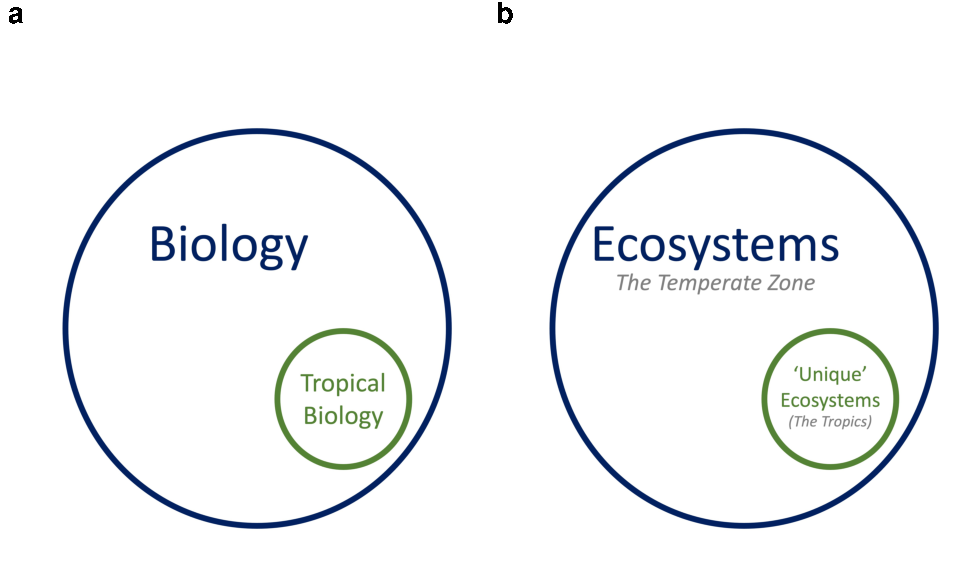
\includegraphics[width=1\linewidth,]{Bruna_plenary_MS_files/figure-latex/fig1-1} 

}

\caption{(A) Tropical biology conceptualized as biological specialization. (B) Tropical ecosystems conceptualized as "unique" or "special".}\label{fig:fig1}
\end{figure}

\begin{figure}[H]

{\centering 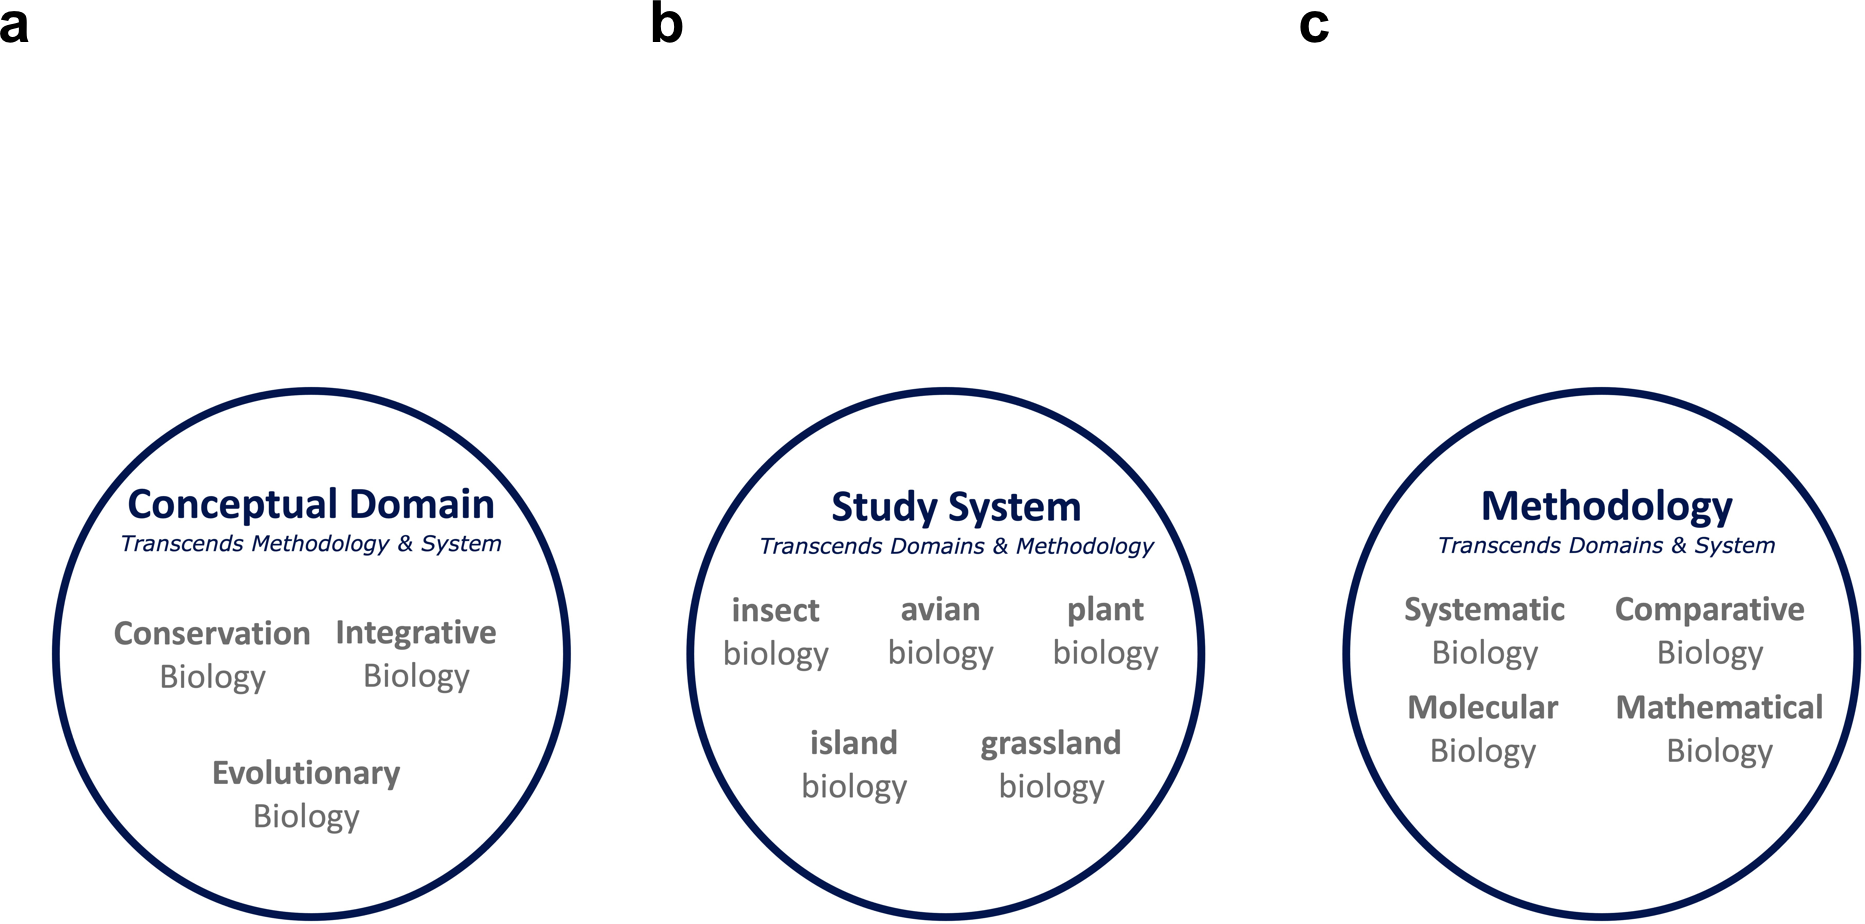
\includegraphics[width=1\linewidth,]{Bruna_plenary_MS_files/figure-latex/fig2-1} 

}

\caption{Alternative ways in Biologists self-organize into specialized subdiciplines: (A) the Conceptual Domain from which they approach their work, (B) their focal Study System, and (C) the Methdological Approaches they use to conduct their research.}\label{fig:fig2}
\end{figure}


\end{document}
